%\RequirePackage[l2tabu, orthodox]{nag}
\documentclass[12pt]{beamer}
\graphicspath{{Imagenes/}{../Imagenes/}}
\usepackage[utf8]{inputenc}
\usepackage[spanish]{babel}
\usepackage[autostyle,spanish=mexican]{csquotes}
\usepackage{hyperref}
\hypersetup{
  colorlinks=true,
  linkcolor=blue,          % color of internal links (change box color with linkbordercolor)
  citecolor=green,        % color of links to bibliography
  filecolor=magenta,      % color of file links
  urlcolor=cyan,           % color of external links
  linkbordercolor={0 0 1}
}
\usepackage{amsmath}
\usepackage{amsthm}
\usepackage{amsfonts}
\usepackage{multicol}
\usepackage{graphicx}
\usepackage{tabulary}
\usepackage{booktabs}
\usepackage{epstopdf}
\usepackage{media9}
\usepackage[binary-units=true]{siunitx}
\usepackage{standalone}
\usepackage{longtable}
\usepackage{bigints}
\usepackage{caption}
%\usepackage{enumitem}
\usepackage{tikz}
\usetikzlibrary{mindmap}
\usepackage[siunitx]{circuitikz}
\usetikzlibrary{arrows, patterns, shapes, decorations.markings}
\usetikzlibrary{matrix,positioning}
\tikzstyle{every picture}+=[remember picture,baseline]
\usepackage{color}
\usepackage{alltt}
\usepackage{verbatim}

\usepackage{fancyvrb}
\usepackage[os=win]{menukeys}
\usepackage{pifont}
\usepackage[sfdefault]{roboto}  %% Option 'sfdefault' only if the base font of the document is to be sans serif
%\usepackage[T1]{fontenc}
\setcounter{secnumdepth}{3}
\setcounter{tocdepth}{3}
\DeclareGraphicsExtensions{.pdf,.png,.jpg}
\renewcommand {\arraystretch}{1.5}
\definecolor{ao}{rgb}{0.0, 0.5, 0.0}
\definecolor{bisque}{rgb}{1.0, 0.89, 0.77}
\definecolor{amber}{rgb}{1.0, 0.75, 0.0}
\definecolor{armygreen}{rgb}{0.29, 0.33, 0.13}
\definecolor{alizarin}{rgb}{0.82, 0.1, 0.26}
\definecolor{cadetblue}{rgb}{0.37, 0.62, 0.63}
\newcommand*{\TitleParbox}[1]{\parbox[c]{6cm}{\raggedright #1}}%
\newcommand{\python}{\texttt{python}}
\newcommand{\textoazul}[1]{\textcolor{blue}{#1}}
\newcommand{\azulfuerte}[1]{\textcolor{blue}{\textbf{#1}}}
\newcommand{\funcionazul}[1]{\textcolor{blue}{\textbf{\texttt{#1}}}}
%\normalfont
\usepackage{ccfonts}% http://ctan.org/pkg/{ccfonts}
\usepackage[T1]{fontenc}% http://ctan.or/pkg/fontenc
\renewcommand{\rmdefault}{cmr}% cmr = Computer Modern Roman
\usefonttheme[onlymath]{serif}
\linespread{1.3}
\newcounter{saveenumi}
\newcommand{\seti}{\setcounter{saveenumi}{\value{enumi}}}
\newcommand{\conti}{\setcounter{enumi}{\value{saveenumi}}}

%reduce el tamaño de letra de la etiqueta equations
\makeatletter
\def\maketag@@@#1{\hbox{\m@th\normalfont\small#1}}
\makeatother

%se usa para la x en itemize
\newcommand{\xmark}{\text{\ding{55}}}

%\AtBeginDocument{\setlength{\tymin}{1em}}


\definecolor{myblue}{rgb}{.8, .8, 1}

\usepackage{amsmath}
\usepackage{empheq}

\newlength\mytemplen
\newsavebox\mytempbox

\makeatletter
\newcommand\mybluebox{%
    \@ifnextchar[%]
       {\@mybluebox}%
       {\@mybluebox[0pt]}}

\def\@mybluebox[#1]{%
    \@ifnextchar[%]
       {\@@mybluebox[#1]}%
       {\@@mybluebox[#1][0pt]}}

\def\@@mybluebox[#1][#2]#3{
    \sbox\mytempbox{#3}%
    \mytemplen\ht\mytempbox
    \advance\mytemplen #1\relax
    \ht\mytempbox\mytemplen
    \mytemplen\dp\mytempbox
    \advance\mytemplen #2\relax
    \dp\mytempbox\mytemplen
    \colorbox{myblue}{\hspace{1em}\usebox{\mytempbox}\hspace{1em}}}

\makeatother

\sisetup{separate-uncertainty}%


%Se usa la plantilla Warsaw modificada con spruce
\mode<presentation>
{
  \usetheme{Warsaw}
  \setbeamertemplate{headline}{}
  \useoutertheme{default}
  %\usecolortheme{beaver}
  \setbeamercovered{invisible}
}
%\AtBeginSection[]
%{
%\begin{frame}<beamer>{Contenido}
%\normalfont\mdseries
%\tableofcontents[currentsection]
%\end{frame}
%}

\setbeamertemplate{section in toc}[sections numbered]
\setbeamertemplate{subsection in toc}[subsections numbered]
\setbeamertemplate{subsection in toc}{\leavevmode\leftskip=3.2em\rlap{\hskip-2em\inserttocsectionnumber.\inserttocsubsectionnumber}\inserttocsubsection\par}
\setbeamercolor{section in toc}{fg=blue}
\setbeamercolor{subsection in toc}{fg=blue}
\setbeamertemplate{navigation symbols}{}
\setbeamercolor{frametitle}{fg=yellow,bg=blue!70!white}
\setbeamercolor{section in head/foot}{bg=gray!30,fg=red}
%\setbeamercolor{section in head}{bg=green,fg=red}
\setbeamercolor{subsection in head/foot}{bg=gray!30,fg=black}
\setbeamercolor{author in head/foot}{bg=gray!30}
\setbeamercolor{date in head/foot}{fg=blue}

%\mode<presentation>
%{
%  \usetheme{Warsaw}
%  \setbeamertemplate{headline}{}
%  %\useoutertheme{infolines}
%  \useoutertheme{default}
%  \setbeamercovered{invisible}
%  % or whatever (possibly just delete it)
%}

%\input{../Preambulos/pre_codigo}
\makeatletter
\setbeamertemplate{footline}
{
  \leavevmode%
  \hbox{%
  \begin{beamercolorbox}[wd=.333333\paperwidth,ht=2.25ex,dp=1ex,center]{author in head/foot}%
    \usebeamerfont{author in head/foot} \insertsection
  \end{beamercolorbox}}%
  \begin{beamercolorbox}[wd=.333333\paperwidth,ht=2.25ex,dp=1ex,center]{title in head/foot}%
    \usebeamerfont{title in head/foot} \insertsubsection
  \end{beamercolorbox}%
  \begin{beamercolorbox}[wd=.333333\paperwidth,ht=2.25ex,dp=1ex,right]{date in head/foot}%
    \usebeamerfont{date in head/foot} \textcolor{white}{\insertshortdate{}} \hspace*{2em}
    \textcolor{white}{\insertframenumber{} / \inserttotalframenumber}\hspace*{2ex} 
  \end{beamercolorbox}}%
  \vskip0pt%
\makeatother
\title{\large{Tema 1 - Conceptos básicos}}
\subtitle{Curso de Física}
\author[]{M. en C. Gustavo Contreras Mayén}
\date{\today}
\institute{Facultad de Ciencias - UNAM}
\titlegraphic{
\includegraphics[width=2cm]{../Imagenes/escudo-facultad-ciencias}\hspace*{4.75cm}~%
   
\includegraphics[width=2cm]{../Imagenes/escudo-unam}
}
\begin{document}
\maketitle
\section*{Contenido}
\frame[allowframebreaks]{\tableofcontents[currentsection, hideallsubsections]}
\fontsize{14}{14}\selectfont
\spanishdecimal{.}
\section{¿Qué estudia la física?}
\frame{\tableofcontents[currentsection, hideothersubsections]}
\subsection{Introducción}
\begin{frame}   
\frametitle{¿Qué estudia la física?}
La física estudia lo grande y lo pequeño, lo viejo y lo nuevo. 
\\
\bigskip
Del átomo a las galaxias, de los circuitos eléctricos a la aerodinámica, la física es una gran parte del mundo que nos rodea.
\end{frame}
\begin{frame}
\frametitle{Reflexión}
Deviene claro que el ulterior progreso en cualquier ciencia es imposible sin la utilización de los logros de otras ramas del conocimiento.
\end{frame}
\begin{frame}
\frametitle{Reflexión}
La matemática y la física. La física y la química. La matemática y la electrónica.
\\
\bigskip
\pause
La simbiosis de estas ciencias exactas, actualmente parece natural, y la física matemática, la química física y la matemática de computación surgidas como resultado de esta simbiosis ya hace mucho que se han convertido en nombres acostumbrados.
\end{frame}
\begin{frame}
\frametitle{Reflexión}
Quiso la suerte que la biología y la medicina no fueran a parar a la categoría de ciencias exactas.
\\
\bigskip
El objeto de estudio de estas ciencias, el organismo vivo, es hasta tal grado complejo y multiforme que no siquiera hoy en día existe la posibilidad de describir con precisión todas sus características y regularidades.
\end{frame}
\begin{frame}
\frametitle{Reflexión}
En el curso de muchos siglos la biología intervenía tan sólo como una ciencia descriptiva y, prácticamente, no explicaba las causas de la mayoría de los fenómenos que transcurren en el organismo vivo.
\end{frame}
\begin{frame}
\frametitle{Reflexión}
La utilización de los logros de la física y de la química ofreció la posibilidad de investigar los fundamentos de la vida a nivel molecular.
\end{frame}
\begin{frame}
\frametitle{Reflexión}
Como resultado de la interpretación de la química y la biología, así como de la física y la biología, se originaron la bioquímica y la biofísica.
\pause
\vfill
K. Bogdánov. El Físico visita al biólogo. Editorial Mir (1986)
\end{frame}
\begin{frame}[plain]
    \begin{figure}
    \includestandalone[scale=0.55]{Figuras/mapamental2}
    \end{figure}
\end{frame}
\begin{frame}
\frametitle{La física en el estudio}
El estudio de la física es también una aventura:
\pause
\setbeamercolor{item projected}{bg=blue!70!black,fg=yellow}
\setbeamertemplate{enumerate items}[circle]
\begin{enumerate}[<+->]
\item A veces frustante.
\item En otras, dolorosa.
\end{enumerate}
\end{frame}
\begin{frame}
\frametitle{Como hacer física}
La física es una ciencia experimental.
\\
\bigskip
A través de la observación de fenómenos naturales, se busca determinar un modelo y los principios que los describen.
\end{frame}
\begin{frame}   
\frametitle{Modelos en física}
Esos modelos se conocen como teorías físicas, si están muy bien establecidos y se usan ampliamente, se le llaman leyes.
\end{frame}
\begin{frame}
\frametitle{Pasos a seguir}
El desarrollo de la ciencias exige creatividad.
\\
\bigskip
\pause
El científico debe aprender a hacer las preguntas adecuadas, a diseñar experimentos para tratar de resolverlas y a deducir conclusiones apropiadas de los resultados.
\end{frame}
\begin{frame}
\frametitle{Usando modelos en física}
En física como en otras ciencias, una primera aproximación de un sistema o fenómeno natural es a través de un modelo.
\\
\bigskip
\pause
Que es una versión simplificada de ese sistema físico, normalmente demasiado complejo como para analizarse con todos sus pormenores.
\end{frame}
\begin{frame}
\frametitle{Consideraciones en los modelos}
Además se establecen una serie de suposiciones tanto matemáticas como físicas, que permiten el estudio del fenómeno.
\\
\bigskip
\pause
No quiere decir que se eviten o se cancelen, \emph{recordemos que será una primera aproximación al estudio del fenómeno}.
\end{frame}
\begin{frame}
\frametitle{Ejemplo de modelo}
\begin{figure}
    \centering
    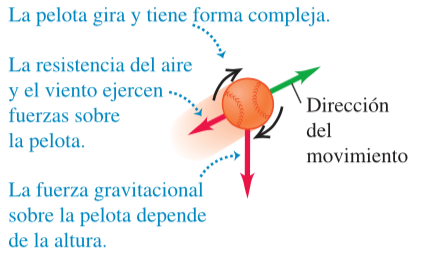
\includegraphics[scale=0.75]{./Imagenes/Modelo_Bola_01.png}
\end{figure}
\end{frame}
\begin{frame}
\frametitle{Ejemplo de modelo}
\begin{figure}
    \centering
    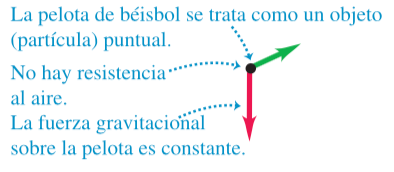
\includegraphics[scale=0.75]{./Imagenes/Modelo_Bola_02.png}
\end{figure}
\end{frame}
\section{Medición e incertidumbre}
\frame{\tableofcontents[currentsection, hideothersubsections]}
\subsection{La medición en Física}
\begin{frame}
\frametitle{Medir en física}
Una de las primeras tareas que debemos de realizar para proponer un modelo a un sistema o fenómeno, es la tarea de medir.
\end{frame}
\begin{frame}
\frametitle{¿Qué es medir?}
De acuerdo a la Real Academia de la Lengua:
\\
\bigskip
\pause
medir:
(\textit{Del lat. metiri.})
\\
\bigskip
1. tr. Comparar una cantidad con su respectiva unidad, con el fin de averiguar cuántas veces la segunda está contenida en la primera.
\end{frame}
\begin{frame}
\frametitle{Cantidades físicas}
Un número empleado para describir cuantitativamente un fenómeno físico se le llama \textcolor{blue}{una cantidad física}.
\\
\bigskip
\pause
Algunas cantidades físicas son tan básicas que sólo podemos definirlas describiendo la forma de medirlas, es decir, con una definición operativa.
\end{frame}
\begin{frame}
\frametitle{Sistema de Medidas}
Al medir una cantidad, \emph{siempre la comparamos con un estándar de referencia}.
\\
\bigskip
\pause
El sistema de unidades empleado por los científicos en todo el mundo se denomina comúnmente \enquote{sistema métrico} aunque, desde 1960, su nombre oficial es \textbf{Sistema Internacional}, o \textbf{SI}.
\end{frame}
\begin{frame}
\frametitle{Unidades base}
Son 7 unidades sobre las que se fundamenta el sistema y de cuya combinación se obtienen todas las unidades derivadas.
\end{frame}
\begin{frame}[plain]
\frametitle{Unidades base}
\begin{tabular}{ | c | c | c |}
\hline
Magnitud & Unidad & Símbolo \\ \hline
\textbf{longitud} & metro & m \\ \hline
\textbf{masa} & kilogramo & kg \\ \hline
\textbf{tiempo} & segundo & s \\ \hline
\textbf{corriente eléctrica} & ampere & A \\ \hline
\textbf{temperatura termodinámica} & kelvin & K \\ \hline
\textbf{intensidad luminosa} & candela & cd \\ \hline
\textbf{cantidad de sustancia} & mol & mol \\ \hline
\end{tabular}
\end{frame}
\begin{frame}[plain]
\frametitle{Metro}
Es la longitud de la trayectoria recorrida por la luz en el vacío en un lapso de 1/299 792 458 de segundo.
\begin{figure}
    \centering
    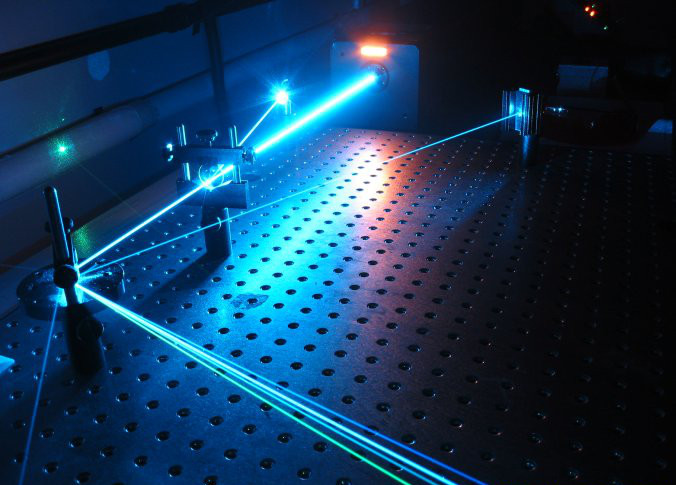
\includegraphics[scale=0.35]{./Imagenes/Lab1Laser.jpg}
\end{figure}
\end{frame}
\begin{frame}[plain]
\frametitle{Masa}
\hspace{-1cm}
\begin{minipage}{5.5cm}
Es la masa igual a la del prototipo internacional del kilogramo: un cilindro de platino iridio de diámetro y altura iguales (39 mm)
\end{minipage}
\hspace{0.75cm}
\begin{minipage}{5cm}
\begin{figure}
    \centering
    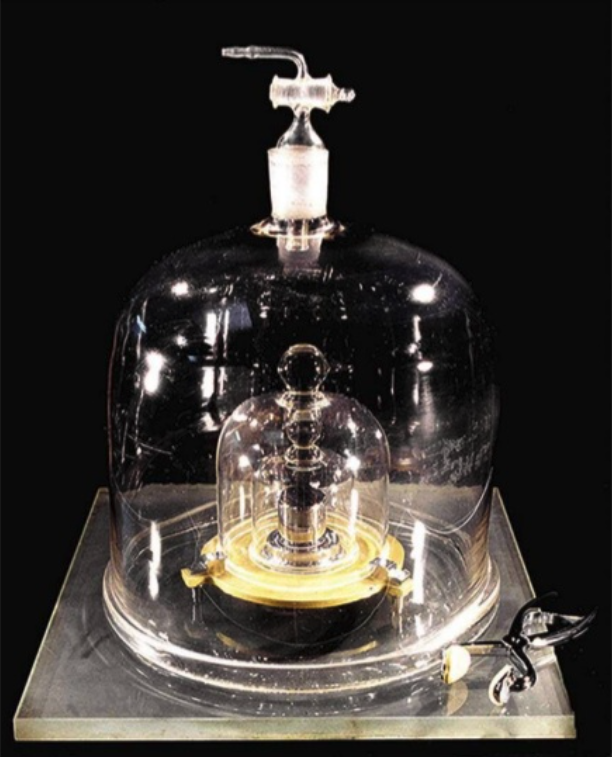
\includegraphics[scale=0.25]{./Imagenes/Masa_Prototipo.png}
\end{figure}
\end{minipage}
\end{frame}
\begin{frame}
\frametitle{Curiosidades sobre el cilindro}
\setbeamercolor{item projected}{bg=blue!70!black,fg=yellow}
\setbeamertemplate{enumerate items}[circle]
\begin{enumerate}[<+->]
\item Se fabricó en 1889.
\item La proporción de platino es del $90\%$ y $10\%$ de iridio.
\item Está resguardado en la Oficina del Buró Internacional de Pesos y Medidas (BIPM)
\item Existen sólo 6 copias oficiales.
\item Se han distribuido $80$ copias en el mundo para adaptarlas como prototipos.
\item El manejo de la campana es extremadamente cuidadoso, ya que evita el contacto con polvo, humedad, etc.
\end{enumerate}
\end{frame}
\begin{frame}[plain]
\frametitle{Segundo}
Es la duración de 9 192 631 770 períodos de la radiación correspondiente a la transición entre los dos niveles hiperfinos del estado fundamental del átomo de cesio 133.
\begin{figure}
    \centering
    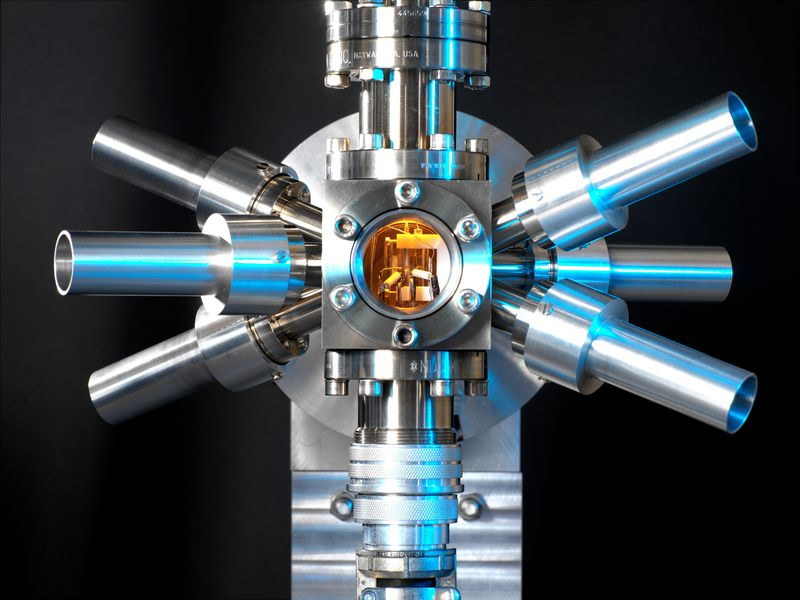
\includegraphics[scale=0.2]{./Imagenes/Reloj_Atomico.jpg}
\end{figure}
\end{frame}
\begin{frame}[plain]
\frametitle{Reloj atómico de cesio}
\begin{figure}
    \hspace*{-1cm}
    \centering
    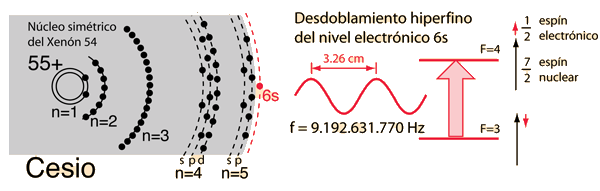
\includegraphics[scale=0.6]{./Imagenes/Csclock.png}
\end{figure}
\end{frame}
\begin{frame}
\frametitle{Ampere}
Es la intensidad de una corriente constante que mantenida en dos conductores paralelos, rectilíneos de longitud infinita, de sección circular despreciable, colocados a un metro de distancia entre sí, en el vacío, producirá entre ellos una fuerza igual a $\SI{2e-7}{\newton\per\metre}$
\end{frame}
\begin{frame}
\frametitle{Kelvin}
Es la fracción de $1/273.16$ de la temperatura termodinámica del punto triple del agua.
\end{frame}
\begin{frame}
\frametitle{Kelvin}
Es de uso común expresar una temperatura termodinámica (\textbf{T}) en función de su diferencia por relación a la temperatura de referencia $T_{0} = \SI{273.15}{\kelvin}$, punto de congelación del agua.
\end{frame}
\begin{frame}
\frametitle{Kelvin}
Esta diferencia de temperatura es llamada temperatura Celsius (\textbf{t}) y se define como
\[ t - T - T_{0} \]
La unidad de temperatura Celsius es el grado Celsius ($\SI{}{\celsius}$) igual a la unidad kelvin por definición.
\end{frame}
\begin{frame}
\frametitle{Candela}
Es la intensidad luminosa en una dirección dada de una fuente que emite una radiación monocromática de frecuencia $\SI{540e12}{\hertz}$ y cuya intensidad energética en esa dirección es $\SI{1/683}{\watt\per\steradian}$.
\end{frame}
\begin{frame}
\frametitle{Esterorradián}
Se define como un ángulo sólido que, teniendo su centro en el de una esfera, tiene una superficie (sobre la esfera) igual al cuadrado del radio. El ángulo sólido de una esfera completa es $4 \: \pi$ estereorradianes.
\begin{figure}
    \centering
    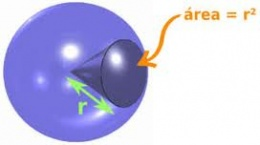
\includegraphics[scale=0.7]{./Imagenes/estereorradian.jpg}
\end{figure}
\end{frame}
\begin{frame}
\frametitle{mol}
Es la cantidad de sustancia que contiene tantas entidades elementales como existen átomos en $\SI{0.012}{\kilogram}$ de carbono 12.
\end{frame}
\begin{frame}
\frametitle{mol}
En general, un mol de cualquier sustancia contiene $\si{6.022e23}$ moléculas o átomos de dicha sustancia.
\\
\bigskip
Así pues, en un mol de agua ($H_{2}O$) hay $\si{6.022e23}$ moléculas de $H_{2}O$.
\end{frame}
\begin{frame}
\frametitle{mol}
En Estados Unidos el \textcolor{blue}{día del mol} se celebra cada 23 de octubre, entre las 6:02 de la mañana y las 6:02 de la tarde aprovechando los dígitos del número de Avogadro.
\end{frame}
% \section{Cinématica}
% \frame{\tableofcontents[currentsection, hideothersubsections]}
% \subsection{Nombre Subseccion}

% \begin{frame}

% \end{frame}


\end{document}